\chapter{Ашкөз алгоритмдер}

\index{ашкөз алгоритмдер}

\key{Ашкөз алгоритм} -- есепті әрдайым 
дәл қазіргі уақытта  тиімді болатын жауапты 
таңдау арқылы шығаратын алгоритм түрі.
Ашкөз алгоритм жасаған шешімдерін қайтармайды,
қарастырылған шешімдердің ең тиімдісінен жауап құрастырады. 
Сол себепті де ашкөз алгоритмдерді әдетте өте
ұтымды таңдау деп есептейді.

Алайда ашкөз алгоритмді жобалаудың өзіндік қиындығы да бар. Ол -- 
есепке әрдайым оңтайлы жауапты 
табатын ашкөз стратегияны құру.
Локалды оңтайлы шешімдер глобалды 
оңтайлы болу керек. Ашкөз алгоритмнің
дұрыс жұмыс жасайтынын дәлелдеу көбіне қиынға соғады.

\section{Тиын жайлы есеп}

Алдымен мысал арқылы қарастырайық:
бізге тиындардың жиыны берілген, қосындысы 
$n$ болатын тиындарды таңдау керек. 
Тиындардың мәндері: $\texttt{coins}=\{c_1,c_2,\ldots,c_k\}$ 
және бір тиынды қалағанымызша алсақ болады.
''Ең аз дегенде қанша тиын қажет?'' - деген сұраққа жауап іздейміз.

Мысалы, $n=520$ және тиындар 
\[\{1,2,5,10,20,50,100,200\}\]
болса, бізге кемінде 4 тиын алу керек.
Бұл жердегі оңтайлы жауап  -- $200+200+100+20(=520)$ тиындарын алу.

\subsubsection{Ашкөз алгоритм}

Бұл есепті шығаратын қарапайым ашкөз алгоритм бізге қажет сома жиналғанға дейін әрдайым мүмкін болатын ең үлкен тиынды алып отырады. Алгоритм бұл мысалда қисынды жұмыс істейді, яғни
басында біз құны 200-дік екі тиынды, одан кейін құны 100-дік бір тиынды аламыз, ал ең соңында құны 20-лық бір тиын алынады. 

Егер тиындарды теңге деп қабылдасақ, онда алгоритміміз \emph{дұрыс}
жұмыс жасайды. Басқаша айтқанда, алгоритм әрдайым
ең аз мөлшерде қолданылатын тиындарды алады. Алгоритмнің
дұрыстығын былай көрсетуге болады:

Біріншіден, әр 1, 5, 10, 50 және 100 тиындары
жауапта ең көп дегенде бір рет кездеседі.
Егер жауапта бірдей тиын екі рет кездессе, 
оларды мәндес бір тиынмен ауыстырып, оңтайлы 
жауап алуға болады. Мысалы, егер жауапта $5+5$ тиындары
болса, оларды $10$ тиынмен ауыстыруға болады.

Дәл солай 2, 20 тиындары ең көп дегенде 2 рет кездеседі,
себебі $2+2+2$ тиындарын $5+1$ тиындарымен, $20+20+20$ 
тиындарын $50+10$ тиындарымен ауыстырса болады. Оған қоса,
оңтайлы жауапта $2+2+1$ және $20+20+10$ тиындары болмайды.
Себебі біз оларды $5$ және $50$ тиындармен ауыстыра аламыз.

Осы бақылауларды қолдана отырып, біз
әрбір $x$ тиыны үшін тек $x$ мәнінен
кіші тиындарды пайдалану арқылы $x$ қосындысын табу
немесе кез келген үлкен соманы оңтайлы түрде құру 
мүмкін еместігін көрсете аламыз. Мысалы, $x=100$
болса, кішкентай тиындарды қолдану арқылы шығатын ең үлкен 
және оңтайлы қосынды $50+20+20+5+2+2=99$ болады. 
Демек әрдайым үлкен тиынды алатын ашкөз алгоритм тиімді
жауап береді. 

Бұл мысал осындай қарапайым ашкөз алгоритмнің 
дұрыс жұмыс істейтінін дәлелдеу қиын екендігін көрсетеді. 

\subsubsection{Жалпы жағдай}

Жалпы жағдайда тиын жиыны әртүрлі тиындырдан тұруы мүмкін
және ашкөз алгоритм міндетті түрде оңтайлы \emph{жауап бермейді}.

Ашкөз алгоритмнің дұрыс жұмыс істемейтінін қарсы 
мысал келтіріп көрсетсек болады. Басқаша айтқанда, алгоритм
қате жауап беретін мысал келтірсек болады.
Мәселен, тиындар $\{1,3,4\}$
және қорытынды қосынды 6 болған жағдайды алайық.
Алгоритм $4+1+1$ жауабын тапқанымен, оңтайлы жауап
$3+3$ болады.

Есептің жалпы барысын шығаратын ашкөз алгоритмнің
болу-болмауы белгісіз\footnote{
Дегенмен ашкөз алгоритмнің берілген тиындардың жиынында 
қалай жұмыс істейтінін полиномдық уақытта \emph{тексеруге} болады
\cite{pea05}.}. Алайда, 7-тарауда, 
кейбір жағдайда бұл есептің жалпы түрін динамикалық бағдарламалау
арқылы дұрыс шығаруға болатынын көреміз.

\section{Жоспарлау}

Көптеген жоспарлау есептерін ашкөз алгоритм 
арқылы шығаруға болады. Көрнекілік үшін классикалық есеп түрін келтірейік:
Бізге $n$ оқиғаның басталуы мен аяқталу уақыттары
берілген. Мүмкіндігінше көп оқиғаларды 
қамтитын жоспарды табыңыз. Бір оқиғаны жартылай алуға
болмайды және алған оқиғалар өзара қиылыспау керек.
Мысалы, төмендегі оқиғаларды қарастырайық:
\begin{center}
\begin{tabular}{lll}
оқиға & басталу уақыты & аяқталу уақыты \\
\hline
$A$ & 1 & 3 \\
$B$ & 2 & 5 \\
$C$ & 3 & 9 \\
$D$ & 6 & 8 \\
\end{tabular}
\end{center}
Бұл жағдайда ең көп оқиғалар саны екіге тең.
Үлгі ретінде $B$ және $D$ оқиғаларын алсақ болады:
\begin{center}
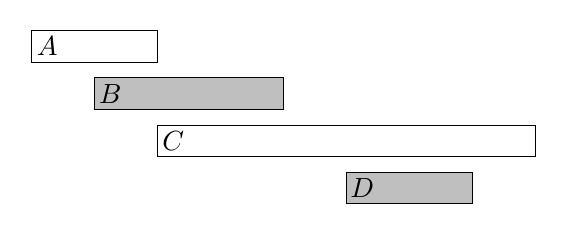
\begin{tikzpicture}[scale=.4]
  \begin{scope}
    \draw (2, 0) rectangle (6, -1);
    \draw[fill=lightgray] (4, -1.5) rectangle (10, -2.5);
    \draw (6, -3) rectangle (18, -4);
    \draw[fill=lightgray] (12, -4.5) rectangle (16, -5.5);
    \node at (2.5,-0.5) {$A$};
    \node at (4.5,-2) {$B$};
    \node at (6.5,-3.5) {$C$};
    \node at (12.5,-5) {$D$};
  \end{scope}
\end{tikzpicture}
\end{center}

Бұл есепті шығаратын бірнеше ашкөз алгоритмдерді
құрастыруға болады. Солардың қайсысы әрдайым дұрыс 
жауапты ұсына алмақ?


\subsubsection*{1-алгоритм}

Бірінші идея -- мүмкіндігінше \emph{қысқа} 
оқиғаларды алу. Бұл жағдай үшін алгоритміміз
келесі оқиғаларды таңдайды:
\begin{center}
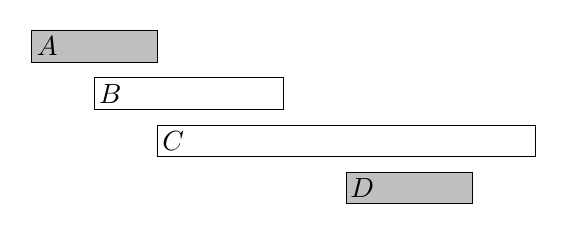
\begin{tikzpicture}[scale=.4]
  \begin{scope}
    \draw[fill=lightgray] (2, 0) rectangle (6, -1);
    \draw (4, -1.5) rectangle (10, -2.5);
    \draw (6, -3) rectangle (18, -4);
    \draw[fill=lightgray] (12, -4.5) rectangle (16, -5.5);
    \node at (2.5,-0.5) {$A$};
    \node at (4.5,-2) {$B$};
    \node at (6.5,-3.5) {$C$};
    \node at (12.5,-5) {$D$};
  \end{scope}
\end{tikzpicture}
\end{center}

Бірақ, қысқа оқиғаларды алу әрдайым оңтайлы бола бермейді.
Мысалы, келесі жағдайда алгоритм қате жауап шығарады:
\begin{center}
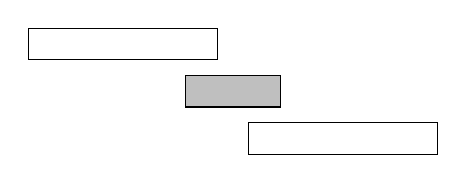
\begin{tikzpicture}[scale=.4]
  \begin{scope}
    \draw (1, 0) rectangle (7, -1);
    \draw[fill=lightgray] (6, -1.5) rectangle (9, -2.5);
    \draw (8, -3) rectangle (14, -4);
  \end{scope}
\end{tikzpicture}
\end{center}
Егер қысқа оқиғаны таңдасақ, нәтижесінде бір ғана оқиғамен қаламыз.
Алайда, тиімді жауап екі ұзын оқиға еді.

\subsubsection*{2-алгоритм}

Келесі идея -- әрдайым  
\emph{ертерек} \emph{басталатын} және алуға мүмкін
оқиғаны таңдау. Бұл алгоритм төмендегідей жұмыс жасайды:
\begin{center}
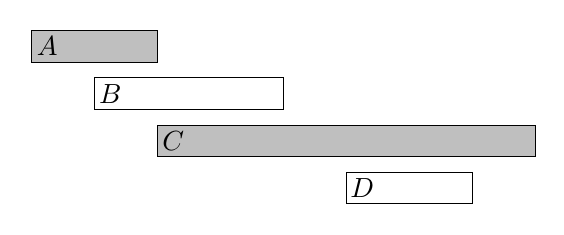
\begin{tikzpicture}[scale=.4]
  \begin{scope}
    \draw[fill=lightgray] (2, 0) rectangle (6, -1);
    \draw (4, -1.5) rectangle (10, -2.5);
    \draw[fill=lightgray] (6, -3) rectangle (18, -4);
    \draw (12, -4.5) rectangle (16, -5.5);
    \node at (2.5,-0.5) {$A$};
    \node at (4.5,-2) {$B$};
    \node at (6.5,-3.5) {$C$};
    \node at (12.5,-5) {$D$};
  \end{scope}
\end{tikzpicture}
\end{center}

Алайда бұл алгоритмге қарсы үлгі таба аламыз.
Мысалы, төмендегі жағдайда алгоритм тек бір оқиғаны 
алады:
\begin{center}
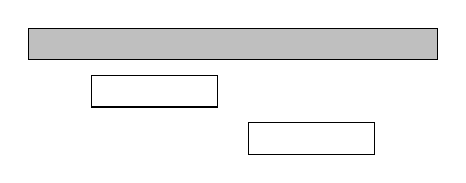
\begin{tikzpicture}[scale=.4]
  \begin{scope}
    \draw[fill=lightgray] (1, 0) rectangle (14, -1);
    \draw (3, -1.5) rectangle (7, -2.5);
    \draw (8, -3) rectangle (12, -4);
  \end{scope}
\end{tikzpicture}
\end{center}
Егер біз бірінші оқиғаны алатын болсақ, онда басқа оқиғаларды
ала алмаймыз. Дегенмен бұл жерде басқа екі оқиғаны алған тиімдірек.

\subsubsection*{3-алгоритм}

Үшінші идея -- қолжетімді ең 
\emph{ерте} \emph{аяқталатын}
оқиғаны алып отыру. Алгоритм төменде келтірілгендей
жұмыс жасайтын болады:
\begin{center}
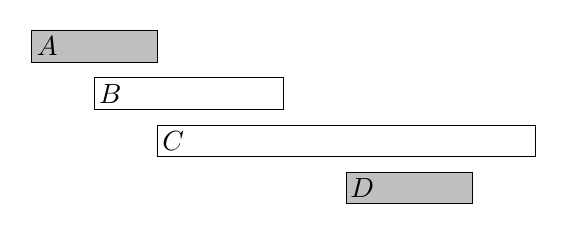
\begin{tikzpicture}[scale=.4]
  \begin{scope}
    \draw[fill=lightgray] (2, 0) rectangle (6, -1);
    \draw (4, -1.5) rectangle (10, -2.5);
    \draw (6, -3) rectangle (18, -4);
    \draw[fill=lightgray] (12, -4.5) rectangle (16, -5.5);
    \node at (2.5,-0.5) {$A$};
    \node at (4.5,-2) {$B$};
    \node at (6.5,-3.5) {$C$};
    \node at (12.5,-5) {$D$};
  \end{scope}
\end{tikzpicture}
\end{center}

Бұл алгоритм \emph{әрдайым} оңтайлы жауап қайтарады. 
Өйткені мүмкіндігінше ерте аяқталатын 
оқиғаны таңдау әрқашан оңтайлы болмақ.
Келесі оқиғаларды да осындай стратегиямен
таңдаймыз, жарамды оқиғалар
таусылғанша осылай жалғастыра береміз.

Бұл алгоритмді дәлелдеу үшін екі оқиғаның
қайсысын таңдау тиімдірек болатынын қарастырайық.
Екеуінен кешірек аяқталатынын таңдасақ,
таңдау саны азаяды. Себебі ол басқа оқиғалардың
алынбауына әсер етеді.
Кеш аяқталатын оқиғаны алу ешқашан тиімді жауап 
бермейді. Сол үшін де жобалаған алгоритміміз дұрыс болмақ.

\section{Тапсырмалар және ақырғы мерзімдер}

Келесі есепті қарастырайық:
Бізге $n$ тапсырмалардың алатын уақыты және
ақырғы мерзімдері берілген. 
Әрбір орындалған тапсырмаға $d-x$ ұпай аламыз,
мұнда $d$ -- тапсырманың ақырғы мерзімі және $x$-тапсырманың 
орындалған уақыты. Тапсырмаларды қандай
ретпен орындау арқылы ең көп ұпай аламыз?

Мысал:
\begin{center}
\begin{tabular}{lll}
тапсырма & алатын уақыты & ақырғы мерзім \\
\hline
$A$ & 4 & 2 \\
$B$ & 3 & 5 \\
$C$ & 2 & 7 \\
$D$ & 4 & 5 \\
\end{tabular}
\end{center}
Бұл кездегі оңтайлы орындау ретіміз төмендегідей болады:
\begin{center}
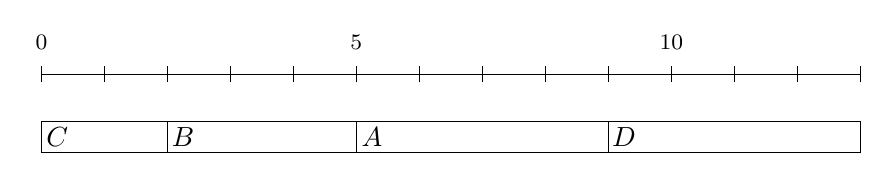
\begin{tikzpicture}[scale=.4]
  \begin{scope}
    \draw (0, 0) rectangle (4, -1);
    \draw (4, 0) rectangle (10, -1);
    \draw (10, 0) rectangle (18, -1);
    \draw (18, 0) rectangle (26, -1);
    \node at (0.5,-0.5) {$C$};
    \node at (4.5,-0.5) {$B$};
    \node at (10.5,-0.5) {$A$};
    \node at (18.5,-0.5) {$D$};

    \draw (0,1.5) -- (26,1.5);
    \foreach \i in {0,2,...,26}
    {
        \draw (\i,1.25) -- (\i,1.75);
    }
    \footnotesize
    \node at (0,2.5) {0};
    \node at (10,2.5) {5};
    \node at (20,2.5) {10};

  \end{scope}
\end{tikzpicture}
\end{center}
Бұл жауапта $C$ тапсырмасы 5 ұпай,
$B$ тапсырмасы 0 ұпай, $A$ тапсырмасы
$-7$ ұпай және $D$ тапсырмасы $-8$ ұпай береді.
Қорытынды ұпай саны -- $-10$.

Қанша таңғаларлық болса да, оңтайлы шешім 
ақырғы мерзімдерге тәуелді емес. Бұл
жердегі дұрыс ашкөз стратегия -- тапсырмаларды
\emph{орындау уақытының өсуі} бойынша атқару.
Оны былай дәлелдей аламыз:
Екі тапсырманы қарастырайық.
Бірінші тапсырманың орындалу уақыты екінші тапсырманың
орындалу уақытынан ұзағырақ.
Егер олардың орындарын ауыстырсақ жауапты тиімдірек 
ете аламыз.
% (Басқаша айтқанда $x1, x2$ тапсырма орындалу және
% $d1, d2$ тапсырмалардың ақырғы уақыты деп белгілейік. 
% $x1 > x2$ деп алсақ, біз $d1-x1 + d2-(x1+x2)$ ұпай аламыз. 
% Бірақ олардың орындарын ауыстырсақ $d1-x2+d2-(x1+x2)$ 
% ұпай аламыз. $d1-x1 + d2-(x1+x2)$ мен $d1-x2 + d2-(x1+x2)$ 
% салыстырсақ оң жақтағы өрнек үлкен болады
% себебі $x1 > x2$. ). 
Осылайша біз орындалу уақыттары қысқа болатын
тапсырмаларды бірінші орындау керектігін дәлелдейміз.
Тағы бір мысал ретінде келесі кестені келтірейік:
\begin{center}
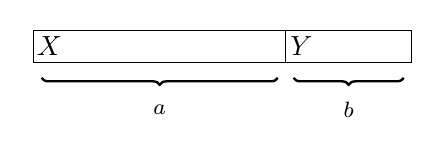
\begin{tikzpicture}[scale=.4]
  \begin{scope}
    \draw (0, 0) rectangle (8, -1);
    \draw (8, 0) rectangle (12, -1);
    \node at (0.5,-0.5) {$X$};
    \node at (8.5,-0.5) {$Y$};

\draw [decoration={brace}, decorate, line width=0.3mm] (7.75,-1.5) -- (0.25,-1.5);
\draw [decoration={brace}, decorate, line width=0.3mm] (11.75,-1.5) -- (8.25,-1.5);

\footnotesize
\node at (4,-2.5) {$a$};
\node at (10,-2.5) {$b$};

  \end{scope}
\end{tikzpicture}
\end{center}
Бұл жерде $a>b$, сол үшін олардың орындарын ауыстыру қажет:
\begin{center}
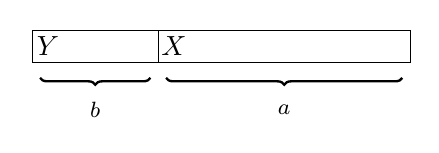
\begin{tikzpicture}[scale=.4]
  \begin{scope}
    \draw (0, 0) rectangle (4, -1);
    \draw (4, 0) rectangle (12, -1);
    \node at (0.5,-0.5) {$Y$};
    \node at (4.5,-0.5) {$X$};

\draw [decoration={brace}, decorate, line width=0.3mm] (3.75,-1.5) -- (0.25,-1.5);
\draw [decoration={brace}, decorate, line width=0.3mm] (11.75,-1.5) -- (4.25,-1.5);

\footnotesize
\node at (2,-2.5) {$b$};
\node at (8,-2.5) {$a$};

  \end{scope}
\end{tikzpicture}
\end{center}
$X$ оқиғасы $b$ ұпай кемітсе, $Y$ оқиғасы $a$ ұпай арттырды.
Қорытынды ұпай саны $a-b > 0$ санына көбейеді.
Оңтайлы шешімде қатарынан келетін әр екі
тапсырма үшін алдымен орындалу уақыты тезірек 
тапсырма атқарылуы қажет.
Сол себепті алгоритмді орындалу уақыты бойынша
сұрыпталған реттілікпен атқарған жөн.

\section{Қосындыны минималдау}

Келесі есепте $n$ сан
$a_1,a_2,\ldots,a_n$ берілген. 
Бізге \[|a_1-x|^c+|a_2-x|^c+\cdots+|a_n-x|^c\]
қосындысы барынша аз болатын $x$ санының
мәнін табу керек.
$c=1$ және $c=2$ жағдайларын ғана қарастырайық.

\subsubsection{$c=1$ жағдайы}

Бұл жағдайда бізге 
\[|a_1-x|+|a_2-x|+\cdots+|a_n-x|\] қосындысын
барынша азайту керек.
Мысалы, сандар $[1,2,9,2,6]$ болса,
оңтайлы жауап $x=2$.
Нәтижесіндегі қосынды:
\[
|1-2|+|2-2|+|9-2|+|2-2|+|6-2|=12.
\]
Жалпы $x$-тің тиімді мәні -- сандардың 
\textit{медианасы} (медиана --
сандарды реттегеннен кейінгі ортаңғы сан).
Мысалы, сандар $[1,2,9,2,6]$ болса,
реттегеннен кейін $[1,2,2,6,9]$ және
медиана 2-ге тең.

Медиана бұл жерде оңтайлы жауап, 
себебі $x$ медианадан аз болса,
$x$-ті арттырумен қосынды азаяды.
Дәл солай $x$ медианадан көп болса да
$x$-ті азайту арқылы қосынды қайтадан азаяды.
Демек оңтайлы жауап $x$-ті медианаға теңеу болып шығады.
Егер $n$ жұп сан болса, онда медиана екеу болады.
Қайсысын алсаңыз да, жауап оңтайлы болады. 

\subsubsection{$c=2$ жағдайы}

Бұл жағдайда бізге \[(a_1-x)^2+(a_2-x)^2+\cdots+(a_n-x)^2\]
қосындысын барынша азайту керек. Мысалы, 
сандар $[1,2,9,2,6]$ болса, оңтайлы жауап
$x=4$ деп алайық. Ол бізге төмендегі қосындыны береді:
\[
(1-4)^2+(2-4)^2+(9-4)^2+(2-4)^2+(6-4)^2=46.
\]
Жалпы $x$-тің оңтайлы мәні -- сандардың
\emph{арифметикалық ортасы}.
Жоғарыда келтірген мысалдағы арифметикалық орта
$(1+2+9+2+6)/5=4$-ке тең.
Осындай нәтижеге қосындыдағы жақшаларды
ашу арқылы қол жеткізуге болады:
\[
nx^2 - 2x(a_1+a_2+\cdots+a_n) + (a_1^2+a_2^2+\cdots+a_n^2)
\]
Соңғы бөлімі $x$-ке тәуелді емес, сондықтан
оны ескермеуге болады.
Ал қалған бөлімдерін $nx^2-2xs$ функциясы ретінде қарастырамыз,
мұндағы $s=a_1+a_2+\cdots+a_n$.
Бұл -- жауаптары $x=0$ және $x=2s/n$ болатын
үстіге ашылған парабола. Параболаның ең кіші мәні --
жауаптарының арифметикалық ортасы $x=s/n$-ге тең,
мұндағы $s=a_1+a_2+\cdots+a_n$.

\section{Деректерді сығымдау}

\index{деректерді сығымдау}
\index{бинарлық код}
\index{код сөз}

\key{Бинарлық код} жолдағы әрбір таңбаға 
биттерден тұратын \key{код сөз} белгілейді.
Жолдағы әрбір таңбаны сәйкес келетін код сөзбен
алмастырып, жолды сығымдауға болады. Мысалы, 
келесі бинарлық код \texttt{A}–\texttt{D} таңбаларына 
код сөз белгілейді:
\begin{center}
\begin{tabular}{rr}
таңба & код сөз \\
\hline
\texttt{A} & 00 \\
\texttt{B} & 01 \\
\texttt{C} & 10 \\
\texttt{D} & 11 \\
\end{tabular}
\end{center}
Бұл -- \emph{тұрақты өлшемді} код
яғни, әрбір код сөздің өлшемі бірдей.
Мысалы, біз \texttt{AABACDACA} жолын
былай сығымдай аламыз:
\[00\,00\,01\,00\,10\,11\,00\,10\,00\]
Осы код арқылы сығымдалған жолдың ұзындығы 
18 бит болады.
Бірақ біз жолдарды \key{айнымалы өлшемді} код 
арқылы тиімдірек сығымдай аламыз. Яғни
код сөздердің өлшемі әртүрлі бола алады. % may have different lengths. note that here we are using бола алады to ensure the word may
Олай болса, көп кездесетін таңбаларға қысқа код
сөзін, ал аз кездесетін таңбаларға ұзын код сөзін
белгілеуімізге болады.
Жоғарыда келтірілген жолға \key{оңтайлы} код төмендегідей  болады:
\begin{center}
\begin{tabular}{rr}
таңба & код сөз \\
\hline
\texttt{A} & 0 \\
\texttt{B} & 110 \\
\texttt{C} & 10 \\
\texttt{D} & 111 \\
\end{tabular}
\end{center}
Оңтайлы код ең қысқа болатын сығымдалған 
жолды береді. 
Жоғарыдағы мысалда оңтайлы код арқылы 
сығымдалған жол:
\[0\,0\,110\,0\,10\,111\,0\,10\,0.\]
Осылайша 18 биттің орнына 15 бит қолдандық. 
Демек жақсы код арқылы сығымдалған жолда 
3 бит сақтауға болады.  

Код сөз басқа код сөздің префиксі 
болмауы -- код сөзге қойылатын басты талап. Мысалы, кодта 10 және
1011 код сөздерінің болуына рұқсат етілмейді.
Себебі сығымдалған жолдан түпкі жолды
өндіруде қиындықтар туындауы мүмкін. 
Егер код сөз басқа код сөздің префиксі болса,
түпкі жолды өндіруе алмаймыз. 
Мысалы, төменде жарамсыз код берілген:
\begin{center}
\begin{tabular}{rr}
таңба & код сөз \\
\hline
\texttt{A} & 10 \\
\texttt{B} & 11 \\
\texttt{C} & 1011 \\
\texttt{D} & 111 \\
\end{tabular}
\end{center}
Кодтағы 1011 сығымдалған жолының түпкі жолы
\texttt{AB} жолы немесе \texttt{C} жолы екені нақты белгісіз.

\index{Хаффман кодтауы}

\subsubsection{Хаффман кодтауы}

\key{Хаффман кодтауы}\footnote{Д.А.Хаффман бұл әдісті 
университеттегі үй жұмысын орындап отырғанда тауып, 
1952 жылы жариялаған. \cite{huf52}.} 
-- жолды сығымдау үшін оңтайлы кодты құрастыратын
ашкөз алгоритм.  
Бұл алгоритм таңбалардың жиілігіне сүйеніп
бинарлы дарақ құрайды. Әр таңбаның
код сөзін дарақтың түбірінен бастап,
жапырағына дейінгі жол арқылы тапсақ болады.
Егер жүрісіміз солға болса, 0 битке, 
оңға болса, 1 битке сәйкес болады.

Бастапқыда жолдың әр таңбасын салмағы таңбаның
жиілігіне тең төбе деп белгілейік. Кейін әр қадам сайын
салмағы ең аз екі төбені алып, олардан салмағы осы
екі төбе салмағының қосындысына тең жаңа
төбе құраймыз. Бұл процесті барлық төбелер 
біріктірілгенше жалғастырамыз.

''\texttt{AABACDACA} жолына
Хаффман кодтауымен қандай оңтайлы код
құрастыра аламыз?'' - деген сұрақ туындайды. 
Басында бізде жолдағы 4 таңбаға сәйкес
4 төбе болады:

\begin{center}
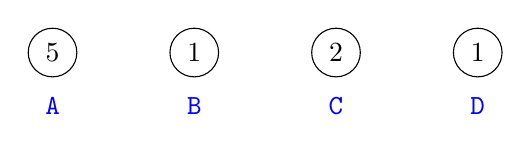
\begin{tikzpicture}[scale=0.9]
\node[draw, circle] (1) at (0,0) {$5$};
\node[draw, circle] (2) at (2,0) {$1$};
\node[draw, circle] (3) at (4,0) {$2$};
\node[draw, circle] (4) at (6,0) {$1$};

\node[color=blue] at (0,-0.75) {\texttt{A}};
\node[color=blue] at (2,-0.75) {\texttt{B}};
\node[color=blue] at (4,-0.75) {\texttt{C}};
\node[color=blue] at (6,-0.75) {\texttt{D}};

%\path[draw,thick,-] (4) -- (5);
\end{tikzpicture}
\end{center}
\texttt{A} таңбасын белгілейтін төбенің салмағы
5, себебі \texttt{A} таңбасы жолда 5 рет кездеседі.
Басқа төбелердің салмақтары да дәл осылай есептеледі.

Бірінші қадамда салмақтары 1 болатын \texttt{B} және 
\texttt{D} сәйкес төбелерін біріктіреміз.

Нәтижесінде:
\begin{center}
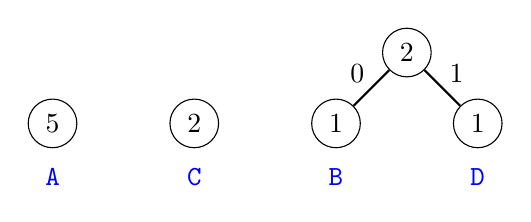
\begin{tikzpicture}[scale=0.9]
\node[draw, circle] (1) at (0,0) {$5$};
\node[draw, circle] (3) at (2,0) {$2$};
\node[draw, circle] (2) at (4,0) {$1$};
\node[draw, circle] (4) at (6,0) {$1$};
\node[draw, circle] (5) at (5,1) {$2$};

\node[color=blue] at (0,-0.75) {\texttt{A}};
\node[color=blue] at (2,-0.75) {\texttt{C}};
\node[color=blue] at (4,-0.75) {\texttt{B}};
\node[color=blue] at (6,-0.75) {\texttt{D}};

\node at (4.3,0.7) {0};
\node at (5.7,0.7) {1};

\path[draw,thick,-] (2) -- (5);
\path[draw,thick,-] (4) -- (5);
\end{tikzpicture}
\end{center}

Бұдан соң салмақтары 2 болатын төбелерді біріктіреміз:
\begin{center}
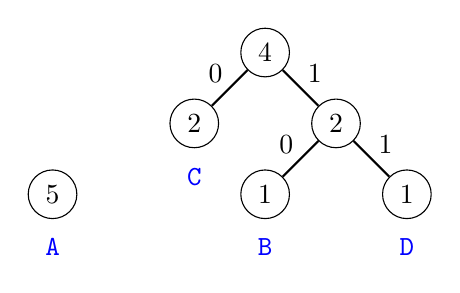
\begin{tikzpicture}[scale=0.9]
\node[draw, circle] (1) at (1,0) {$5$};
\node[draw, circle] (3) at (3,1) {$2$};
\node[draw, circle] (2) at (4,0) {$1$};
\node[draw, circle] (4) at (6,0) {$1$};
\node[draw, circle] (5) at (5,1) {$2$};
\node[draw, circle] (6) at (4,2) {$4$};

\node[color=blue] at (1,-0.75) {\texttt{A}};
\node[color=blue] at (3,1-0.75) {\texttt{C}};
\node[color=blue] at (4,-0.75) {\texttt{B}};
\node[color=blue] at (6,-0.75) {\texttt{D}};

\node at (4.3,0.7) {0};
\node at (5.7,0.7) {1};
\node at (3.3,1.7) {0};
\node at (4.7,1.7) {1};

\path[draw,thick,-] (2) -- (5);
\path[draw,thick,-] (4) -- (5);
\path[draw,thick,-] (3) -- (6);
\path[draw,thick,-] (5) -- (6);
\end{tikzpicture}
\end{center}
Ақырында соңғы екі төбені біріктіреміз:
\begin{center}
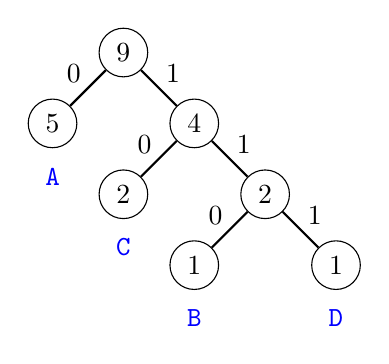
\begin{tikzpicture}[scale=0.9]
\node[draw, circle] (1) at (2,2) {$5$};
\node[draw, circle] (3) at (3,1) {$2$};
\node[draw, circle] (2) at (4,0) {$1$};
\node[draw, circle] (4) at (6,0) {$1$};
\node[draw, circle] (5) at (5,1) {$2$};
\node[draw, circle] (6) at (4,2) {$4$};
\node[draw, circle] (7) at (3,3) {$9$};

\node[color=blue] at (2,2-0.75) {\texttt{A}};
\node[color=blue] at (3,1-0.75) {\texttt{C}};
\node[color=blue] at (4,-0.75) {\texttt{B}};
\node[color=blue] at (6,-0.75) {\texttt{D}};

\node at (4.3,0.7) {0};
\node at (5.7,0.7) {1};
\node at (3.3,1.7) {0};
\node at (4.7,1.7) {1};
\node at (2.3,2.7) {0};
\node at (3.7,2.7) {1};

\path[draw,thick,-] (2) -- (5);
\path[draw,thick,-] (4) -- (5);
\path[draw,thick,-] (3) -- (6);
\path[draw,thick,-] (5) -- (6);
\path[draw,thick,-] (1) -- (7);
\path[draw,thick,-] (6) -- (7);
\end{tikzpicture}
\end{center}

Дарақтағы барлық төбелер біріктірілді. Демек 
кодымыз дайын. 
Дарақтан таңбаларға сәйкес код сөздерді біле аламыз. Олар:
\begin{center}
\begin{tabular}{rr}
таңба & код сөз \\
\hline
\texttt{A} & 0 \\
\texttt{B} & 110 \\
\texttt{C} & 10 \\
\texttt{D} & 111 \\
\end{tabular}
\end{center}
